\documentclass[]{article}

\usepackage[left=0.5in, right=0.5in, top=0.5in, bottom=0.5in]{geometry}
\usepackage{hyperref}
\usepackage{graphicx}
\usepackage{xcolor}
\usepackage{listings}
\usepackage{subcaption}

\colorlet{mygray}{black!30}
\colorlet{mygreen}{green!60!blue}
\colorlet{mymauve}{red!60!blue}

\lstset{
	basicstyle=\ttfamily,
	columns=fullflexible,
	breakatwhitespace=false,      
	breaklines=true,                
	captionpos=b,                    
	commentstyle=\color{mygreen}, 
	extendedchars=true,              
	frame=single,                   
	keepspaces=true,             
	keywordstyle=\color{blue},      
	language=c++,                 
	numbers=none,                
	numbersep=5pt,                   
	numberstyle=\tiny\color{blue}, 
	rulecolor=\color{mygray},        
	showspaces=false,               
	showtabs=false,                 
	stepnumber=5,                  
	stringstyle=\color{mymauve},    
	tabsize=3      
}

\setlength\parindent{0pt}

\hypersetup{
	colorlinks=true,
	linkcolor=blue,
	filecolor=blue,      
	urlcolor=blue
}

% Default fixed font does not support bold face
\DeclareFixedFont{\ttb}{T1}{txtt}{bx}{n}{12} % for bold
\DeclareFixedFont{\ttm}{T1}{txtt}{m}{n}{12}  % for normal

% Custom colors
\usepackage{color}
\definecolor{deepblue}{rgb}{0,0,0.5}
\definecolor{deepred}{rgb}{0.6,0,0}
\definecolor{deepgreen}{rgb}{0,0.5,0}

% Python style for highlighting
\newcommand\pythonstyle{\lstset{
		language=Python,
		basicstyle=\ttfamily,
		otherkeywords={self},             % Add keywords here
		keywordstyle=\color{deepblue},
		emph={MyClass,__init__},          % Custom highlighting
		emphstyle=\color{deepred},    % Custom highlighting style
		stringstyle=\color{deepgreen},
		frame=single,                         % Any extra options here
		showstringspaces=false            % 
}}

% Python for external files
\newcommand\pythonexternal[2][]{{
		\pythonstyle
		\lstinputlisting[#1]{#2}}}

%opening
\title{Automated Plant Care}
%\author{Justin Herter} 
\date{}

\begin{document}

\maketitle

\section{Introduction}
The goal of this project is to implement reliable automation for plant care.  Taking care of plants that yield something of value to the caretaker or his or her employer boils down to supplying the proper levels of light, hydration, and nutrients.  Of these, the first two typically require the caretaker's attention at least once per day.  The most severe potential consequence of neglect is, of course, death of the plant, which renders the entire effort futile.
\\\\
The situation at hand involves a chronically negligent plant caretaker coupled with a low-light environment due to a large bush obstructing the only window.  What is documented here are the steps involved to establish a back-end for the automation itself that is paired with an informative front-end that also sends alerts for key events, e.g. a malfunctioning pump.

\section{System Overview}
The two fundamental pieces of equipment are the light and the pump, and what they both have in common is that they run on AC power.  Obviously, the controller for all of this -- a Raspberry Pi -- is only equipped to handle DC circuits at either 3.3 or 5 volts.  While it's possible to do something with relays, nobody wants to explain their neat project to an angry fire marshal.  Thus, for safety reasons, it has been elected to use a radio frequency (RF) transmitter paired with RF outlet switches to enable switching of the pump and light.  This has an added benefit of greater freedom for routing power.  The remainder of equipment to be used is given in the table below, and Fig. \ref{fig:schematic} provides the \textit{initial} schematic of the design.

\begin{table}[h]
\centering
\caption{Equipment specifications for plant care and monitoring.}
\begin{tabular}{l|l|r }
\textbf{Item} & \textbf{Purpose} & \textbf{Seller or Spec} \\ \hline
AC outlet switches & Allow RF control of AC appliances & \href{https://www.amazon.com/gp/product/B00DQELHBS/ref=ppx_yo_dt_b_search_asin_title?ie=UTF8\&psc=1}{Amazon} \\ \hline
Hygrometer & Monitoring of soil moisture & \href{https://www.aliexpress.com/item/32700826684.html?spm=a2g0s.9042311.0.0.770c4c4dQ7v1Z2}{AliExpress} \\ \hline 
Pump & Supply water to plant & \href{https://www.amazon.com/gp/product/B00EWENMAU/ref=ppx_yo_dt_b_search_asin_title?ie=UTF8&psc=1}{Amazon} \\ \hline 
Light & Provide correct spectrum for plant & Erligpowht 45 W grow light \\ \hline
Photoresistor & Ensure light is operating & GM5539 \\ \hline
Raspberry Pi & Runs at least the back-end & Raspberry Pi 3B \\ \hline
Raspberry Pi camera & Visual of plant and maybe time-lapse & V2 \\ \hline
Arduino Uno & Report analog sensor data & \href{https://www.amazon.com/gp/product/B015QUPO5Y/ref=ppx_yo_dt_b_search_asin_title?ie=UTF8&psc=1}{Amazon} 
\end{tabular}
\end{table}

\subsection{Operation}
The most trivial part of how the system will operate pertains to the light, which will run on a 12 hour on/off schedule.  Half-way through the day portion, the Raspberry Pi will take a still image of the plant.  The photoresistor will be used to ensure the light is working as it should.
\\\\
Next up is the pump operation.  When the hygrometer indicates dry soil, the pump will operate for a brief TBD interval.  This pump will be submerged in a reserve of water that will have a simple circuit that's nominally closed by the water itself until the reserve is nearing depletion.

\subsection{Front-End Requirements}
The front-end will provide a simple, vertically scrolling interface with metrics about delivery of light and water to the plant in the form of two time-series plots for the last 24 hours.  Vertical axes will be the light level from the photoresistor and the moisture level from the hygrometer, respectively.
\\\\
Below the plots, there will be status indicators for the light level, moisture level, and water reserve level.  These will be boolean in nature, and the plant care-taker shall be notified in some way when one of these strays from nominal.  At the bottom of the interface, the most recent picture of the plant will be displayed.
\\\\
Hosting of the front-end will be on an AWS instance running an AMI generated by Packer and provisioned via Terraform.  On this instance, a web server and a database will run in Docker containers orchestrated by Docker Compose.  The web page will be open to the web, and everything else will only be open to the public IP of where the Pi is located.

\section{Sensors and Circuits}
\subsection{RF Outlets}
The starting point is to establish RF capability between the Pi and the RF outlets, which was accomplished by following the steps put forth by GitHub user timeland's \href{https://timleland.com/wireless-power-outlets/}{blog post} and the associated repository \href{https://github.com/timleland/rfoutlet}{rfoutlet}.  The basic procedure is to use an RF receiver to decode signals from the remote that came with the outlets, then use the RF transmitter to emulate the signal for a given channel.  This yielded the codes given in the table below, and Fig. \ref{fig:rf_circuit} shows the setup used.  Also, since it's not explicitly called out, the transmitter and receiver use wiring pi pins zero and two, respectively.  


\begin{table}[h]
\centering
\caption{Codes transmitted by RF outlet remote.}
\begin{tabular}{l|r|r}
	\textbf{Channel} & \textbf{On} &	\textbf{Off}
\\ \hline
	1 &	1398067	& 1398076
\\ \hline
	2 &	1398211	& 1398220
\\ \hline
	3 &	1398531 &1398540
\\ \hline
	4 &	1400067 &1400076
\\ \hline
	5 &	1406211	& 1406220\\
\end{tabular}	
\end{table}

\begin{figure}[h]
	\centering
	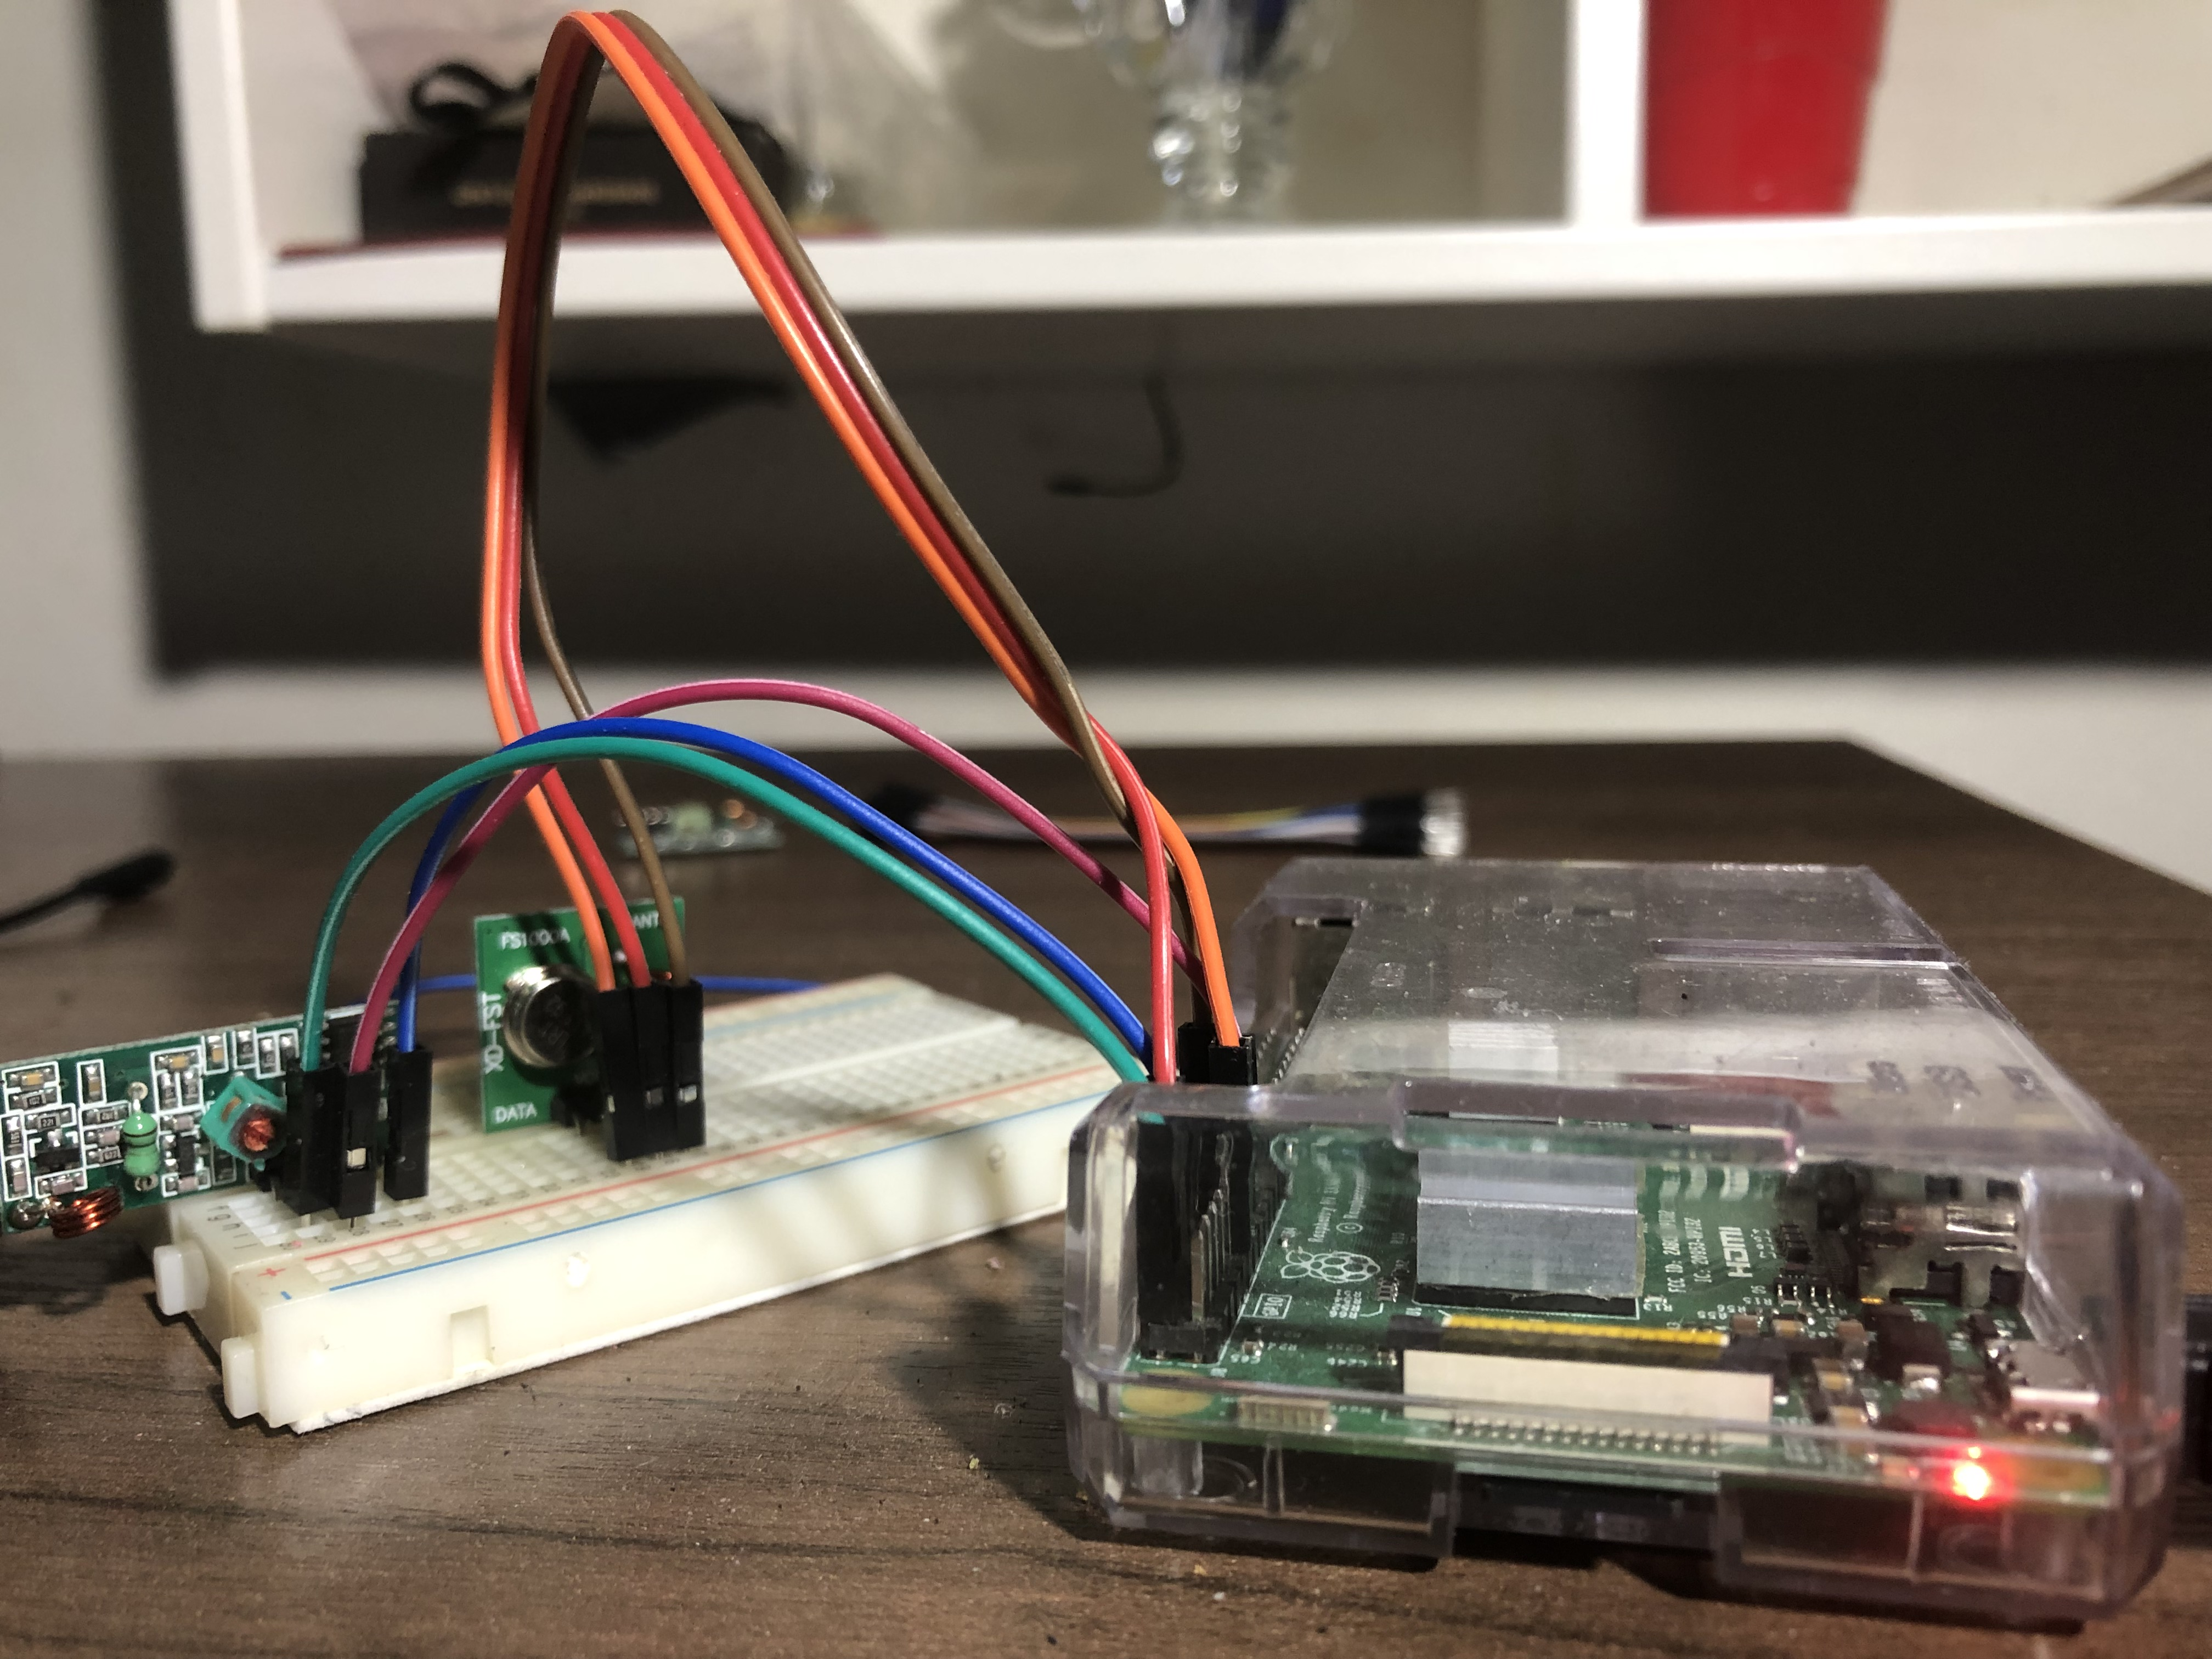
\includegraphics[width=0.5\textwidth]{rf_circuit}
	\caption{Setup for getting RF codes.}
	\label{fig:rf_circuit}
\end{figure}

\subsection{Photoresistor}
A key detail is that a photoresistor is an analog device.  Solutions for the Pi tended to involve capacitors that were not immediately available, so it was decided to use an Arduino Uno to handle analog inputs.  Viewable in Fig. \ref{fig:photoresistor_circuit}, the circuit for the photoresistor is a simple voltage divider, with one side wired to pin A0 and the other being a 10k $\Omega$ resistor leading to ground.  
\\\\
From here, using the Arduino IDE's serial monitor/plotter, it was verified that this arrangement yielded higher values with more light.  It is worth noting that shadows cast substantially affect readings, so the sensor will have to be located in a place that won't be obstructed by leaves.

\begin{figure}
	\centering
	\begin{subfigure}{0.48\textwidth}
		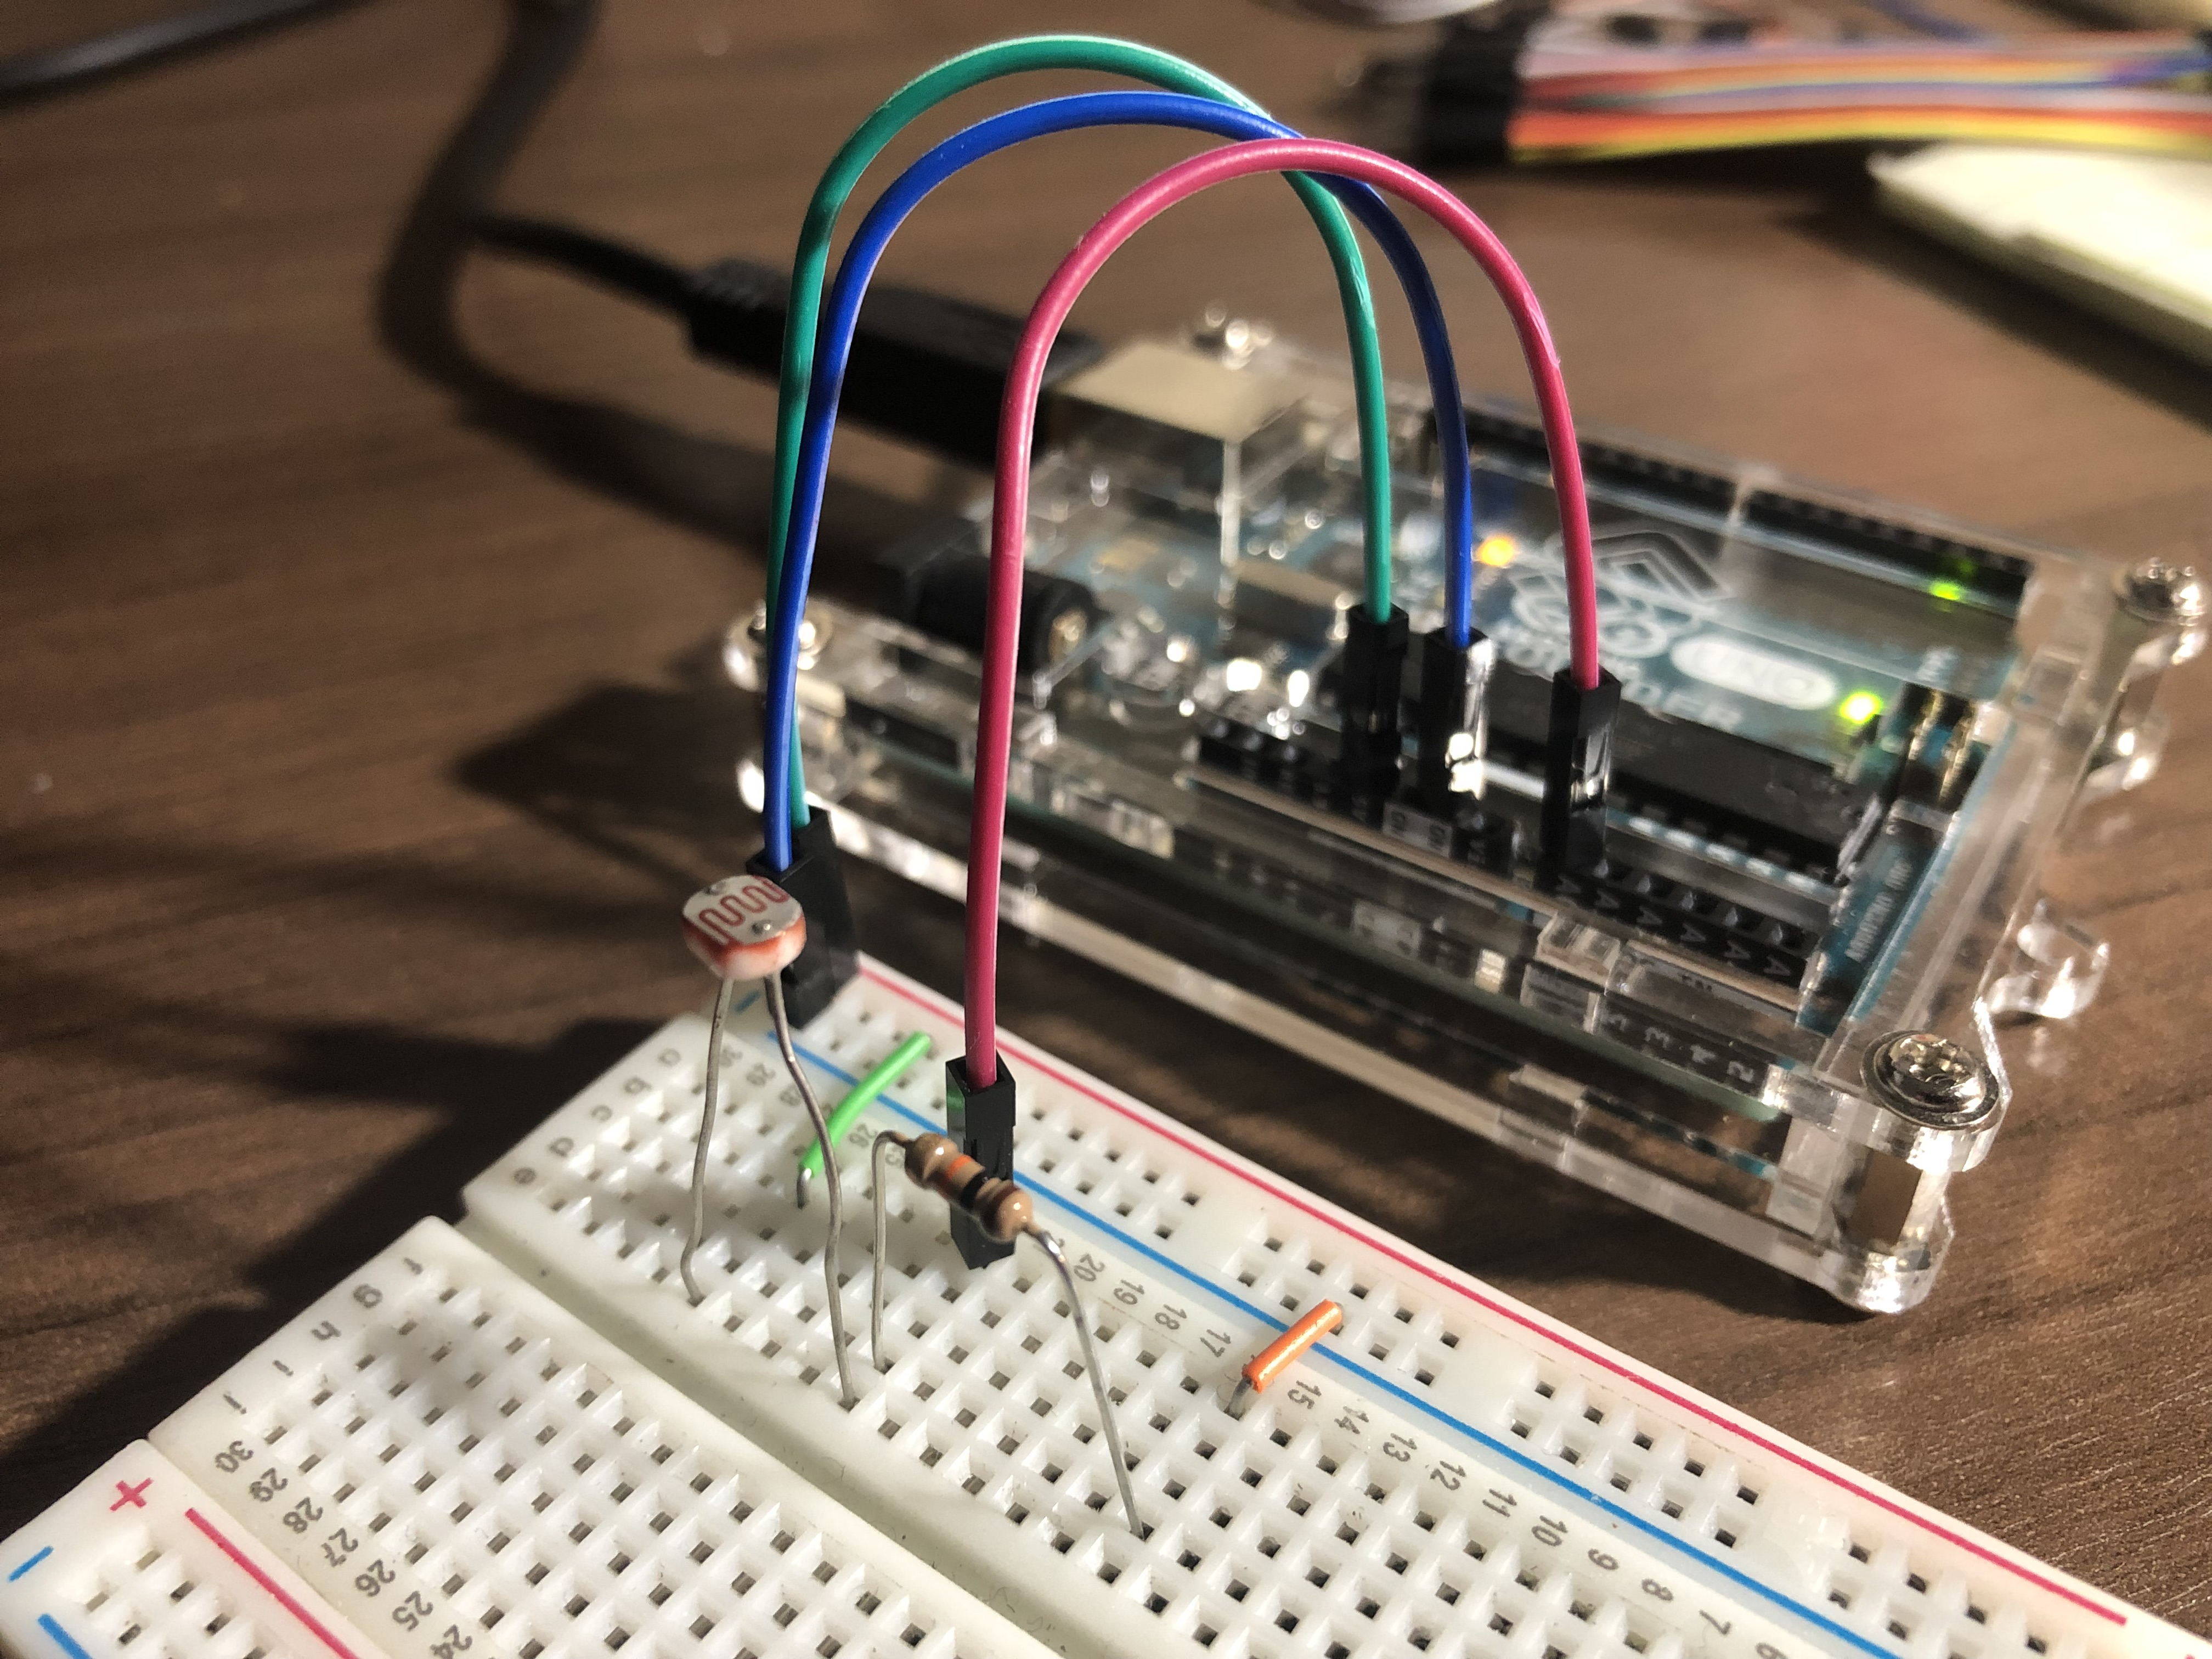
\includegraphics[width=\textwidth]{photoresistor_circuit}
		\caption{Photoresistor circuit.}
		\label{fig:photoresistor_circuit}
	\end{subfigure}
	\begin{subfigure}{0.48\textwidth}
		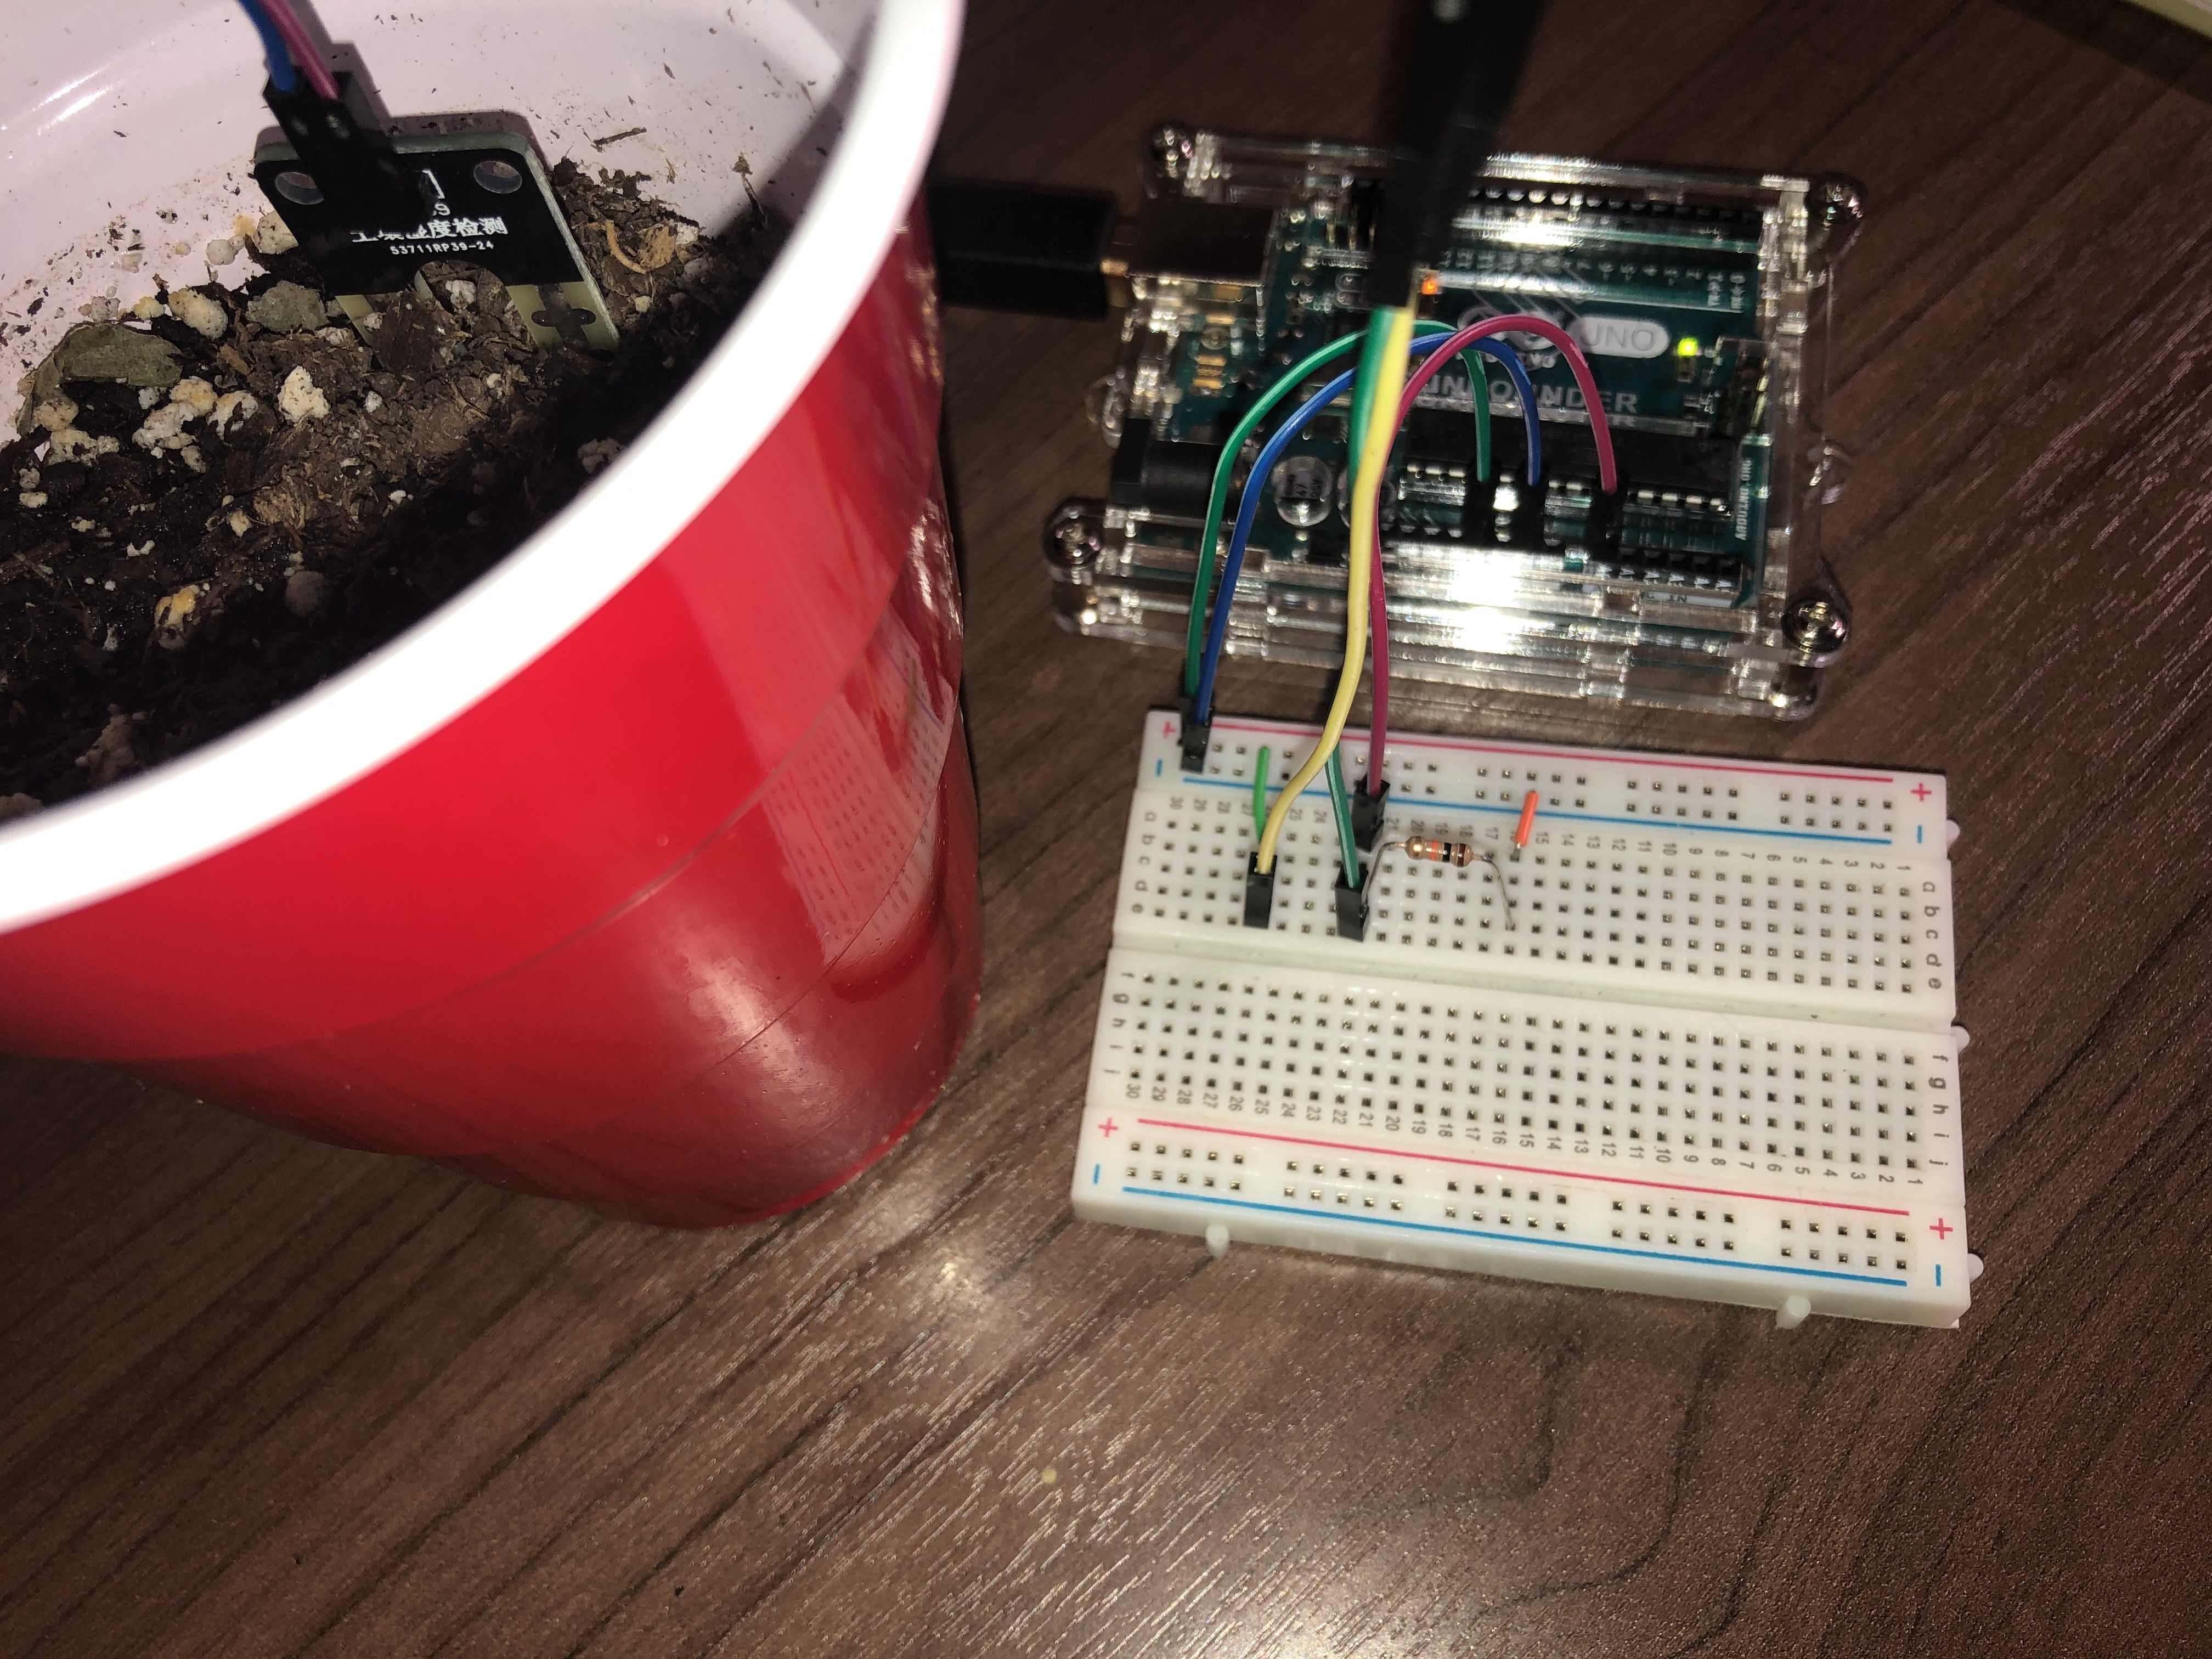
\includegraphics[width=\textwidth]{hygrometer_circuit}
		\caption{Hygrometer circuit.}
		\label{fig:hygrometer_circuit}
	\end{subfigure}
	\caption{Test circuits for analog sensors.}
\end{figure}

\subsection{Hygrometer}
The hygrometers purchased on Ali Express came with a small chip containing a potentiometer that converts the analog signal to a binary, digital one.  The intended use is to set the potentiometer to a threshold value that would serve as a set-point for watering.  
\\\\
For this case, a low/high sensor isn't terribly interesting, so per Fig. \ref{fig:hygrometer_circuit}, the photoresistor was swapped with the hygrometer in a cup of dry soil.  To test the sensor, water was poured into the cup.  Fig. \ref{fig:moisture_plot} shows the serial plotter output for pouring a small bit of water followed by a sustained pour.  By this metric, it seems feasible to incorporate the hygrometer as an analog device, which enables more interesting plots versus time than the digital option.
\begin{figure}[h]
	\centering
	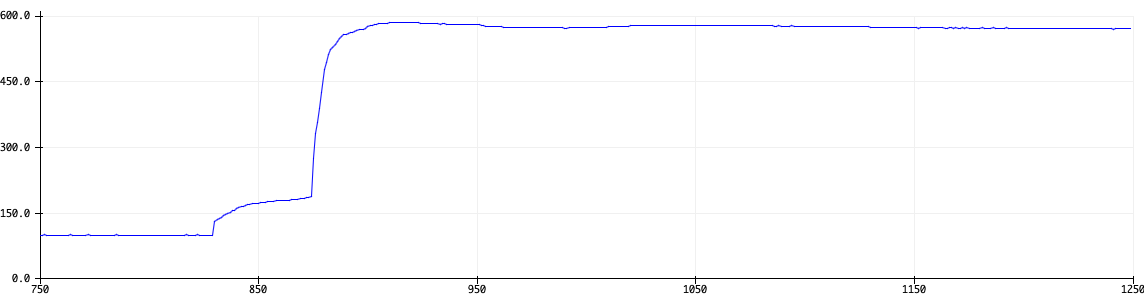
\includegraphics[width=\textwidth]{moisture_plot}
	\caption{Soil moisture versus time (arbitrary units) as water was poured into the cup.}
	\label{fig:moisture_plot}
\end{figure}

\subsection{Water Level}
This is certainly the easiest of the sensors to describe and implement.  Similar to the others, a voltage divider will be used.  When the leads are submerged in the water, the circuit is closed with negligible resistance, so the only change to the general circuit in use is to have another 10k $\Omega$ resistor placed in series with the analog pin to avoid a short.  Given the trivial nature of the sensor, it was not deemed necessary to test this circuit separate from the others.

\newpage
\subsection{Summary and Combined Operation}
Investigating use of a photoresistor, hygrometer, and a simple water level sensor led to a few key findings.  The most significant is that an Arduino is needed to bridge the gap between analog and the Raspberry Pi.  Along with this, it was found that the same basic circuit -- a voltage divider with a 10k $\Omega$ resistor on ground -- can be employed for all three sensors.
\\\\
These criteria informed the writing of the sketch shown in Fig. \ref{fig:arduino_sketch}, which simply prints the state of the three pins delimited by commas.  It is thought best to keep the Arduino sketch dead simple, because there's not a lot to work with as far as libraries or computing power.  Pin mapping is given in the table below.

\begin{table}[h]
	\centering
	\caption{Arduino pin mapping.}
	\begin{tabular}{l|r|r}
		\textbf{Pin} & \textbf{Sensor} \\ \hline
		A0 & Photoresistor \\ \hline
		A1 & Hygrometer \\ \hline
		A2 & Reserve Water Level
	\end{tabular}	
\end{table}

From here, the Raspberry Pi can fetch sensor data as needed over a USB connection.  Fig. \ref{fig:arduino_python_read} shows the Python script that was used to test this combined functionality, and the physical setup given in Fig. \ref{fig:combined_test_circuit} was used to successfully test analog sensing and RF outlet switching.

\begin{figure}[h]
	\centering
	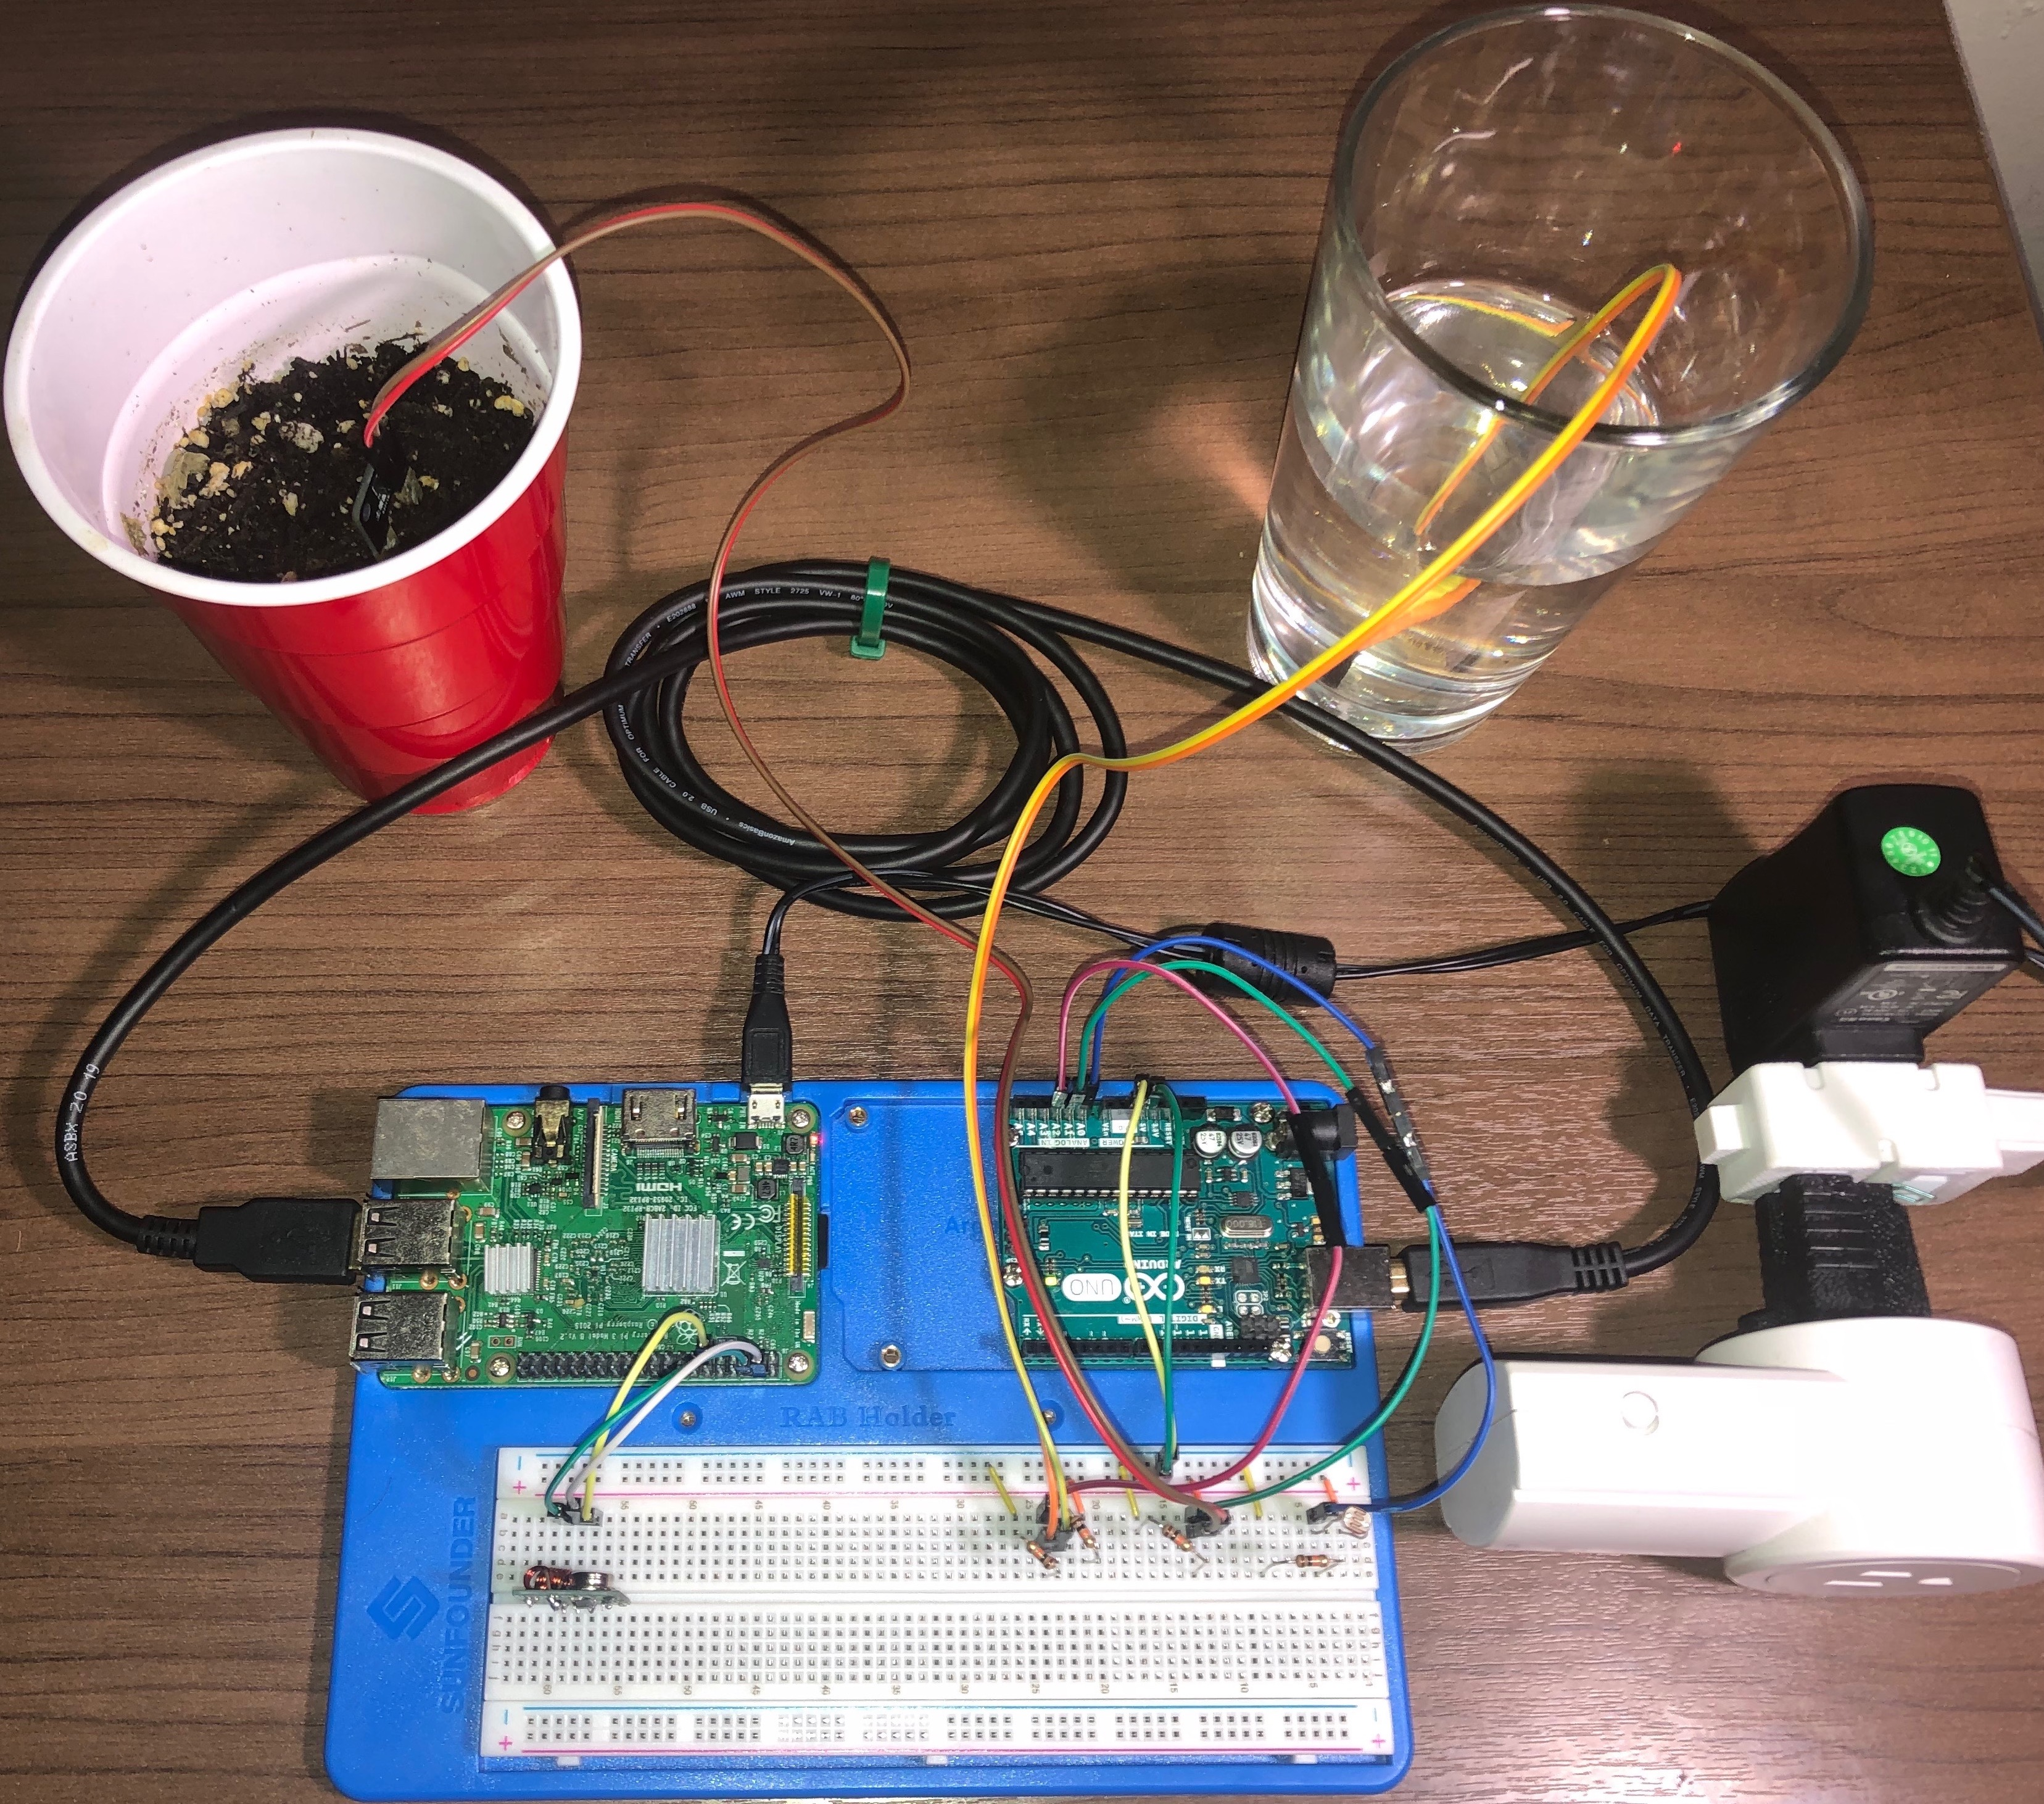
\includegraphics[width=0.9\textwidth]{combined_test_circuit}
	\caption{Combined test setup for analog sensing and RF outlet switching.}
	\label{fig:combined_test_circuit}
\end{figure}

\newpage

\section{Software Design}
For any project, it's best to start with, considering the required inputs and outputs for, in this case, the Raspberry Pi.  Inputs are sensor data from the Arduino, the current time, and camera stills.  Local outputs are RF outlets for the light and pump.  Outputs to a remote host include historic sensor data and the latest image from the camera.
\\\\
Given what's known so far, it seems safe to say that this is an \href{https://www.techopedia.com/definition/7083/event-driven-program}{event-driven program}.  The table below summarizes the anticipated events and the envisioned response from the program.
\begin{table}[h]
	\centering
	\caption{Summary table of event logic.}
	\label{tab:event_response}
	\begin{tabular}{l|r}
		\textbf{Event} & \textbf{Response} \\ \hline
		Light not detected when ``on" & Light status to error \\ \hline
		Soil dry after pump run & Pump status to error \\ \hline
		Reserve level reads low & Warn low reserve level \\ \hline
		Dry soil & Run pump for interval \\ \hline
		Local time 8 am & Turn on light \\ \hline
		Local time 2 pm & Take still image \\ \hline
		Local time 8 pm & Turn off light \\ \hline
	\end{tabular}	
\end{table}

\subsection{Tooling}
A significant design question is the choice of language -- either Python or C++ with Boost.  The biggest pro for Python is a much lower barrier to entry per Fig. \ref{fig:arduino_python_read}, but what's most appealing about C++ is the option to integrate new code with what's in place for controlling the RF outlets.  Given that and Fig. \ref{fig:arduino_sketch}, this choice would also mean that the entire project is written in the same language, and just a single program would have to be run on the Pi.  
\\\\
This tips the scales in favor of C++ with Boost in spite of the added nuance.  Libraries exist for \href{https://www.boost.org/doc/libs/1_65_0/doc/html/boost_asio/overview/serial_ports.html}{serial communication}, and the camera can be accessed using the built-in executable \verb|raspistill|.  To take advantage of new features in \verb|std::filesystem| and similar, C++ 17 has been elected as the project standard.

\begin{table}[h]
	\centering
	\caption{Summary of C++ tooling on the Raspberry Pi.}
	\begin{tabular}{l|r}
		\textbf{Tool} & \textbf{Version} \\ \hline
		make & 4.2.1 \\ \hline
		g++ & 8.3.0 \\ \hline
		gdb & 8.2.1 \\ \hline		
		CMake & 3.15.2 \\ \hline
		Boost & 1.67
	\end{tabular}	
\end{table}

\subsection{Implementation}
Since Raspbian ships with the executable \verb|raspistill|, there's no sense in writing redundant code, so pictures are obtained by invoking \verb|raspistill| via \verb|std::system|.  The actual starting point, however, was the Boost serial library followed by a search for examples on how to use it.  Implemented types are as follows.

\paragraph{SimpleSerial}
This type is a wrapper of what's needed to read serial input asynchronously.  The example this was drawn upon had a reasonable implementation for reading a single line, so a parsing function to convert the string into a vector containing the three expected integers was added.

\paragraph{OutletController}
Methods contained in this type provide an interface to turn the light on or off as well as cycling the pump for a specific number of seconds.  The syntax for actually transmitting a code is wrapped up in \verb|send_code|.

\paragraph{PlantWatcher}
Per its name, this type is responsible for monitoring and orchestrating the respective events and responses detailed in Table \ref{tab:event_response} by interfacing with \verb|SimpleSerial| via \verb|update_sensor_data()| and by having a pet instance of 
\\
\verb|OutletController| to operate on.  Last of all, the method \verb|update_photo()| ensures that a still image is captured and stored a the appropriate time.

% Requires knowledge of systems admin, devops, c++ including cmake, python, circuits.  Had to start with existing code and add functionality

\newpage
\section{Front-End Implementation}


\newpage
\section{Appendix}

\begin{figure}[h]
	\centering
	\includegraphics[height=0.6\textwidth,angle=90]{schematic}
	\caption{Initial schematic of plant automation system.}
	\label{fig:schematic}
\end{figure}

\newpage

\begin{figure}[h]
	\lstinputlisting{../arduino/sketch.cpp}
	\caption{Arduino sketch for reading the photoresistor, hygrometer, and water level sensor.}
	\label{fig:arduino_sketch}
\end{figure}

\newpage

\begin{figure}[h]
	\pythonexternal{../python/arduino_test_read.py}
	\caption{Simple script to test parsing Arduino sensor data on the Raspberry Pi.}
	\label{fig:arduino_python_read}
\end{figure}

\end{document}
